%%%%%%%%%%%%%%%%%%%%%%%%%%%%%%%%%%%%%%%%%%%%%%%%%%%%%%%%%%%%%%%%%%%%%%
% https://www.overleaf.com/9239625sdykfpbkgqxv#/33299142/
% Overleaf (WriteLaTeX) Example: Molecular Chemistry Presentation
%
% Source: http://www.overleaf.com
%
% In these slides we show how Overleaf can be used with standard
% chemistry packages to easily create professional presentations.
%
% Feel free to distribute this example, but please keep the referral
% to overleaf.com
%
%%%%%%%%%%%%%%%%%%%%%%%%%%%%%%%%%%%%%%%%%%%%%%%%%%%%%%%%%%%%%%%%%%%%%%
% How to use Overleaf:
%
% You edit the source code here on the left, and the preview on the
% right shows you the result within a few seconds.
%
% Bookmark this page and share the URL with your co-authors. They can
% edit at the same time!
%
% You can upload figures, bibliographies, custom classes and
% styles using the files menu.
%
% If you're new to LaTeX, the wikibook is a great place to start:
% http://en.wikibooks.org/wiki/LaTeX
%
%%%%%%%%%%%%%%%%%%%%%%%%%%%%%%%%%%%%%%%%%%%%%%%%%%%%%%%%%%%%%%%%%%%%%%

\documentclass{beamer}

% For more themes, color themes and font themes, see:
% http://deic.uab.es/~iblanes/beamer_gallery/index_by_theme.html
%
\mode<presentation>
{
  \usetheme{Madrid}       % or try default, Darmstadt, Warsaw, ...
  \usecolortheme{default} % or try albatross, beaver, crane, ...
  \usefonttheme{serif}    % or try default, structurebold, ...
  \setbeamertemplate{navigation symbols}{}
  \setbeamertemplate{caption}[numbered]
}

\usepackage[english]{babel}
\usepackage[utf8x]{inputenc}
\usepackage{chemfig}
\usepackage[version=3]{mhchem}

% On Overleaf, these lines give you sharper preview images.
% You might want to `comment them out before you export, though.
\usepackage{pgfpages}
\pgfpagesuselayout{resize to}[%
  physical paper width=8in, physical paper height=6in]

% Here's where the presentation starts, with the info for the title slide
\title[Columbia University]{Analysis of U.S. Regional Crime Rates}
\author{Ziwei Meng, Ao Liu}
%\institute{}
\date{\today}

\begin{document}

\begin{frame}
  \titlepage
\end{frame}

% These three lines create an automatically generated table of contents.
\begin{frame}{Outline}
  \tableofcontents
\end{frame}

\section{Overview}
\subsection{Goal and Procedure}
\begin{frame}{Goal and Procedure}
\begin{itemize}
\item Compute the regression model based on the training set and test the accuracy of the model using the test data.
\item Based on the model, implement policies that will lead to the reduction of the number of serious crimes in their county.
\item Discuss the future improvements of the model.
\end{itemize}
\end{frame}


\section{Model Building}
\subsection{Data Overview}
\begin{frame}[fragile]
\frametitle{Data Overview}
\begin{itemize}
\item \textbf{Geographic Data:} Land Area, Geographic Region
\item \textbf{Demographic Data:} Total population, Percent of population aged 18-34, Percent Bachelor’s Degree
\item \textbf{Economics Data:} Percent Below Poverty Level, Total Personal Income, Per Capita Income
\end{itemize}
\end{frame}

\subsection{Data Processing}
\begin{frame}[fragile]
\frametitle{Data Processing}
\begin{itemize}
\item Check for missing values (and substitute them with mean values)
\item Calculate more variables that cater to our needs:\\
(1) Population Density = $\frac{Population}{Area}$\\
(2) Physician Per 1000 Population = $\frac{Population}{Area}$\\
(3) Hospital Beds Per 1000 Population = $\frac{Hospital Beds}{Population/1000}$\\
(4) Crime Rate Per 1000 Population = $\frac{Crimes}{Population/1000}$
\item Randomly Select 330 rows of data to train the regression model, and the remaining 110 rows are used for testing the accuracy of our model
\end{itemize}
\end{frame}

\subsection{Heatmap}
\begin{frame}[fragile]
\frametitle{Heatmap}
First we explore the correlation of variables:
\begin{center}
  \makebox[\linewidth]{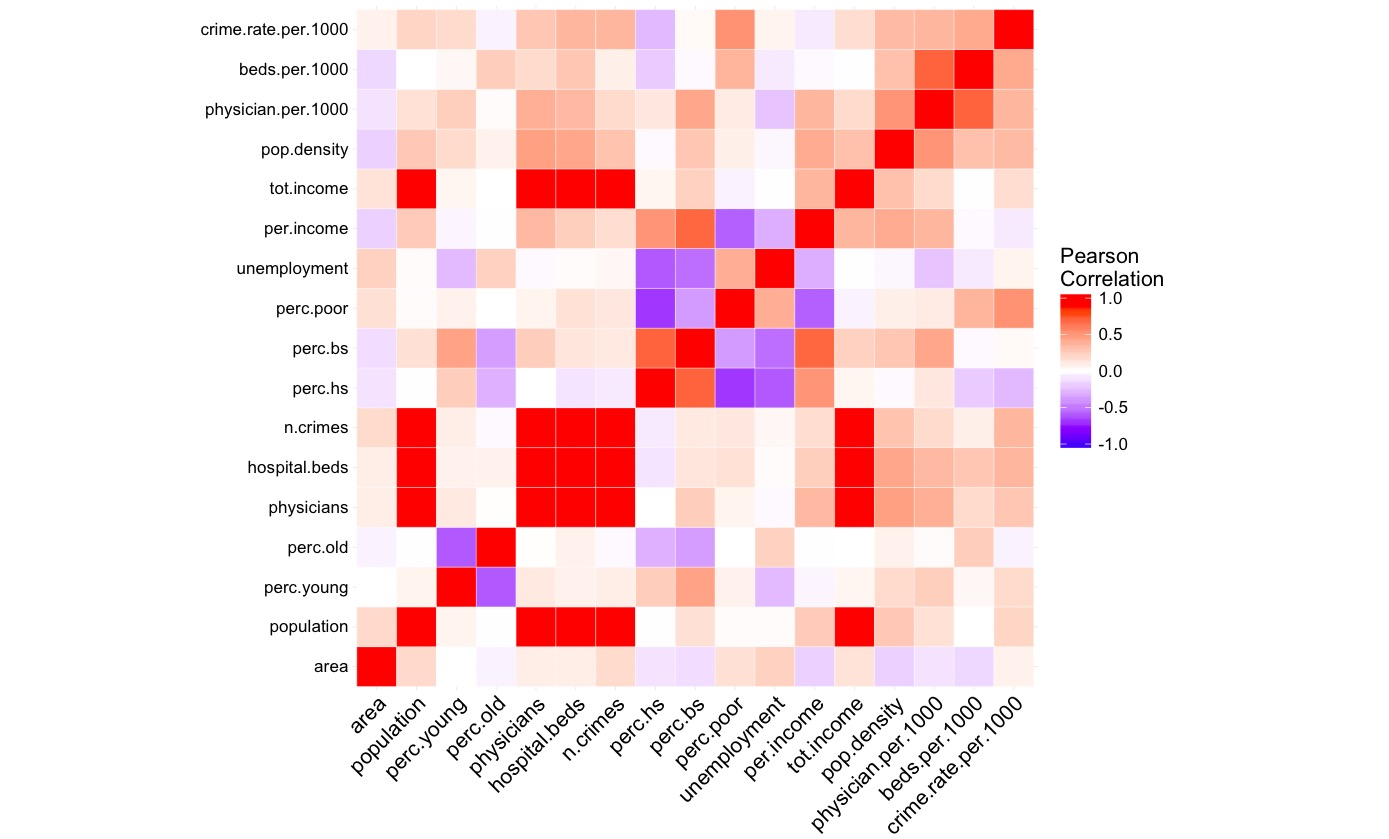
\includegraphics[width=5in]{ada1.jpg}}
\end{center}
\end{frame}

\begin{frame}[fragile]
\frametitle{Heatmap}
\begin{itemize}
\item Given 16 predictor variables, some of them are strongly correlated with each other, which will cause us to get some potentially false conclusion, thus we remove these variables.
\item The remaining variables are:\\
\textsl{Area, Percentage of Young People, Percentage of Old People, Percentage of High School, Percentage of Bachelor, Percentage of Poor, Unemployment, Income,  Region, Population Density, Physician Per 1000 Population, Beds Per 1000 Population}
\end{itemize}
\end{frame}


\subsection{Regression Model}
\begin{frame}[fragile]
\frametitle{Regression Model}
\begin{itemize}
\item Given the fact that crime rate is a value between 0 and 1, using an ordinary linear regression model will affect model's accuracy, in this question we fit the data to \textbf{Poisson Regression Model with Offset and Quasi-likelihood}
\item Then we do the significant test for each variable, and remove the insignificant variables, then do the regression again.
\end{itemize}

\end{frame}


\begin{frame}[fragile]
\frametitle{Outliers}
Check outliers

\begin{center}
  \makebox[\linewidth]{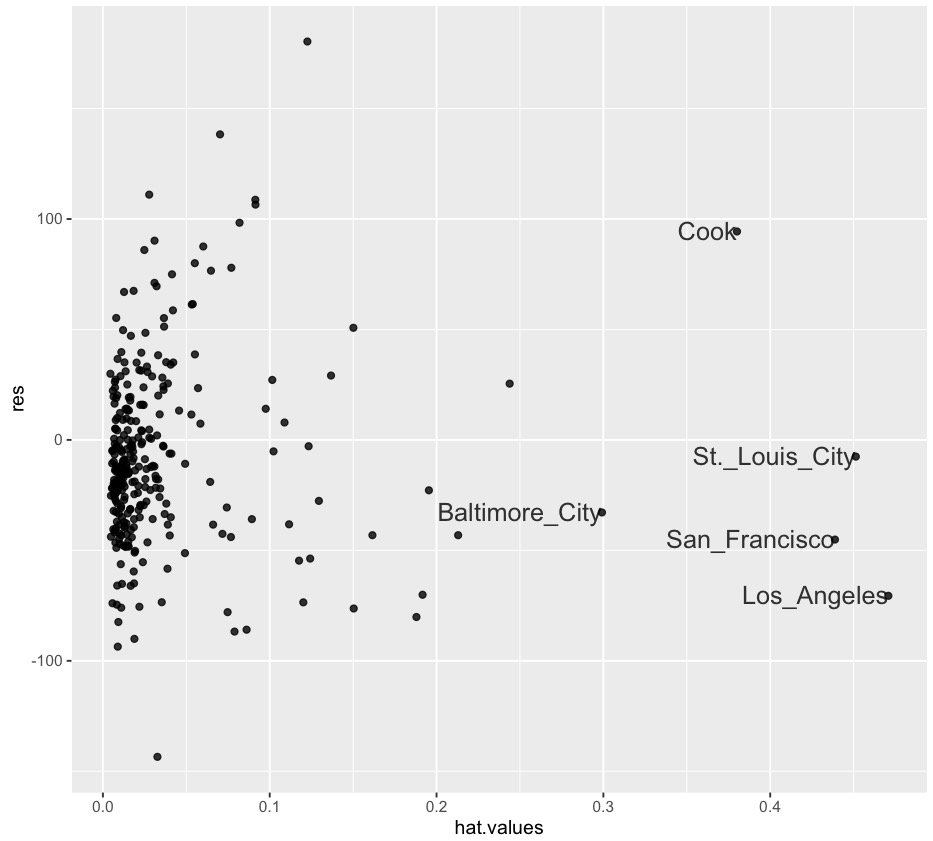
\includegraphics[width=3.2in]{ada2.jpg}}
\end{center}

\end{frame}


\begin{frame}[fragile]
\frametitle{Removal of Insignificant Variables}

\begin{itemize}
\item Through the resulting output table from Poisson Regression, the following variables are insignificant:\\
\textsl{area, percent of old people, percent of people with high school education.}
\item After removing the insignificant variables, we build the Poisson Regression Model again using only the most important variables.
\end{itemize}
\end{frame}



\subsection{Interpretation of Parameters and Visualization}
\begin{frame}[fragile]
\frametitle{Interpretation of Parameters and Visualization}
Here we interpret the meaning of each parameters in our model:\\
\begin{itemize}
\item percent young:
If we increase the percent on young people by 1 while holding all other variables the same, the crime rate would increase by a multiplicative factor of 1.017847 on average.\\
\item percent poor: If we increase the percent on poor people by 1 while holding all other variables the same, the crime rate would increase by a multiplicative factor of 1.024423 on average\\
\item population density: If we increase the log of the population density by 1 while holding all other variables the same, the crime rate would increase by a multiplicative factor of 1.085662 on average.\\
\end{itemize}
\end{frame}


\subsection{Interpretation of Parameters and Visualization}
\begin{frame}[fragile]
\frametitle{Interpretation of Parameters and Visualization}
\begin{itemize}
\item region: Holding all other variables the same, the crime rate in NC is higher than that in NE by a multiplicative factor of 1.347162 on average, the crime rate in S is higher than that in NE by a multiplicative factor of 1.775532 on average, the crime rate in NC is higher than that in W by a multiplicative factor of  on average.\\
\item beds per 1000 population: If we increase the density of beds per 1000 people by 1 while holding all other variables the same, the crime rate would increase by a multiplicative factor of 1.049475 on average.
\end{itemize}
\end{frame}


\begin{frame}[fragile]
\frametitle{Prediction on Testing Data}
\begin{itemize}
\item Finally we use the testing data to predict the crime rate of the remaining 110 counties and examine the accuracy of the regression model
\end{itemize}
\begin{center}
  \makebox[\linewidth]{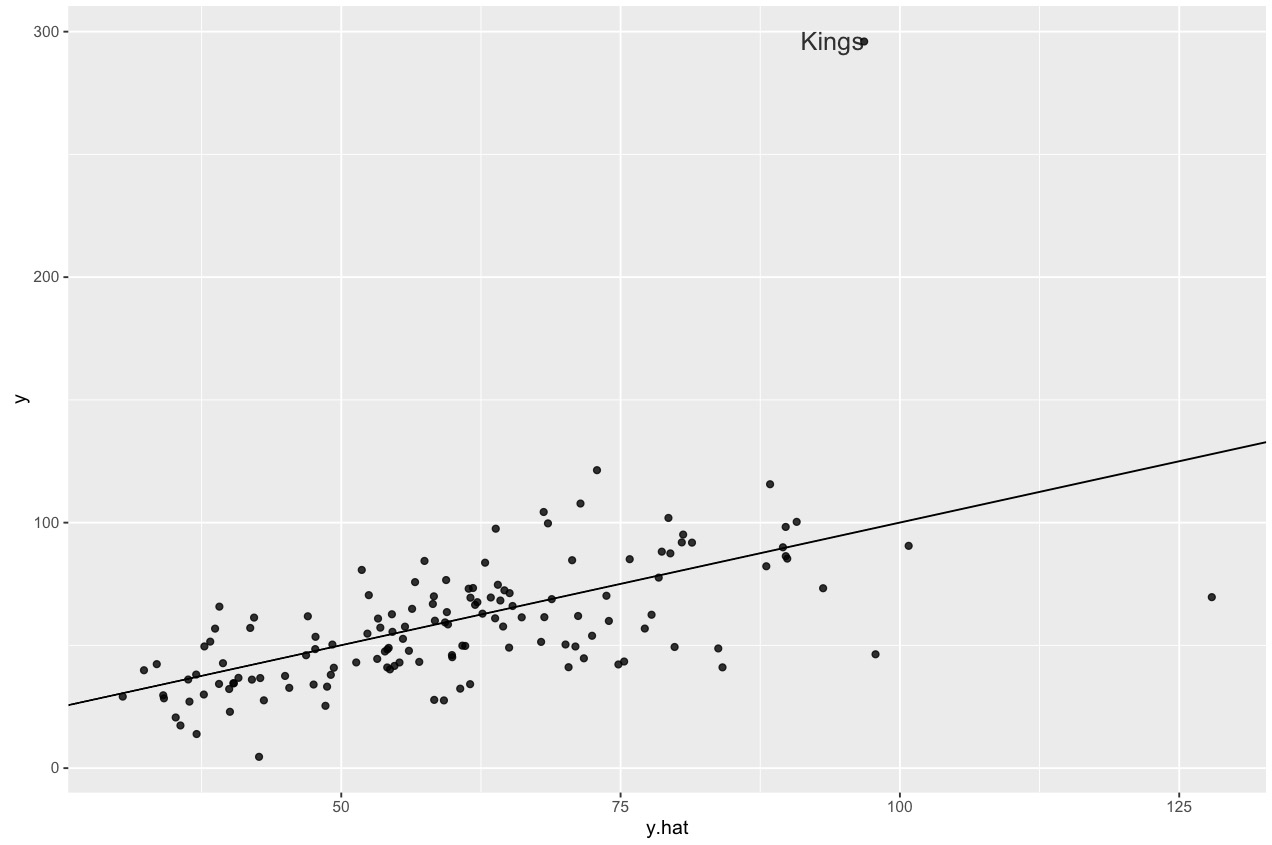
\includegraphics[width=3.2in]{ada3.jpg}}
\end{center}
\end{frame}


\subsection{Random Forest/XGboost Model}
\begin{frame}[fragile]
\frametitle{Random Forest/XGboost Model}
To further explore the data, we fit our data into Random Forest/XGboost Model:
\begin{center}
  \makebox[\linewidth]{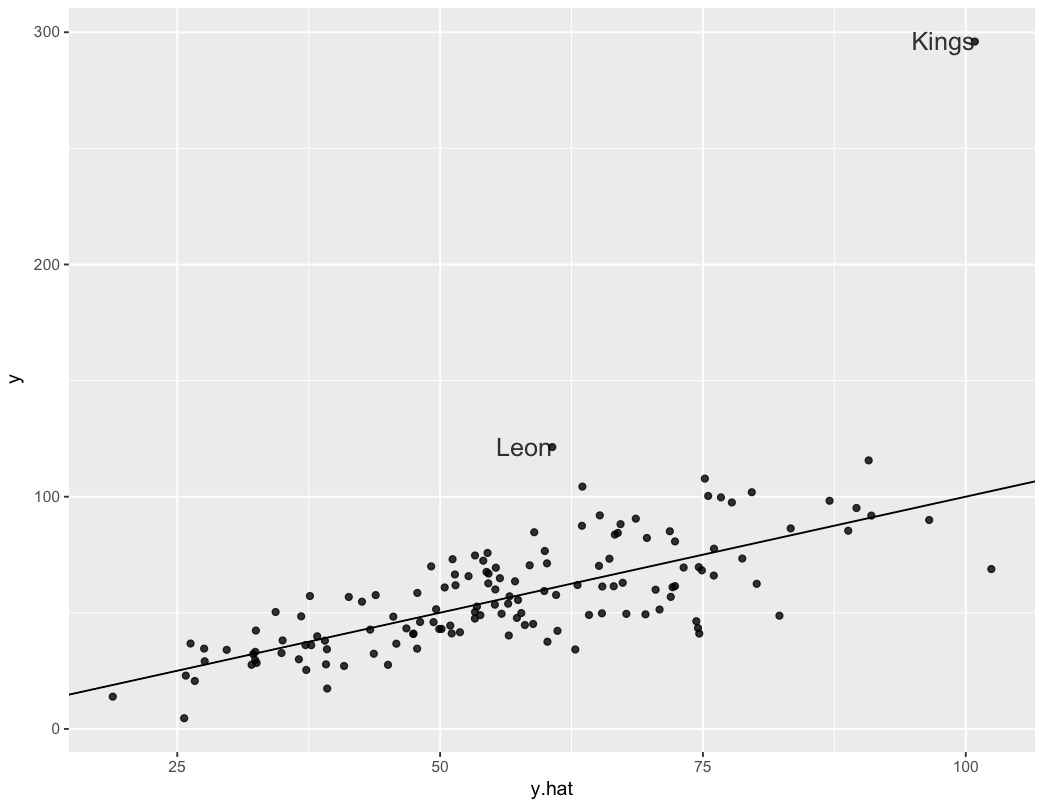
\includegraphics[width=3in]{ada4.jpg}}
\end{center}
\end{frame}




\begin{frame}{Discoveries from the Testing Result}
\begin{itemize}
\item The two models both fit the data well
\item Only several points are outliers, which we don't know the exactly reason for their high crime rate
\item Since our client - Kings County is also among the several outliers in both models, we have to do further analysis to find out the hidden reason for its high crime rate. Otherwise, our suggestions may not be applicable to Kings County.
\end{itemize}

\end{frame}


\begin{frame}[fragile]
\frametitle{Most Important Variables}
Let's see what are the most important variables:
\begin{center}
  \makebox[\linewidth]{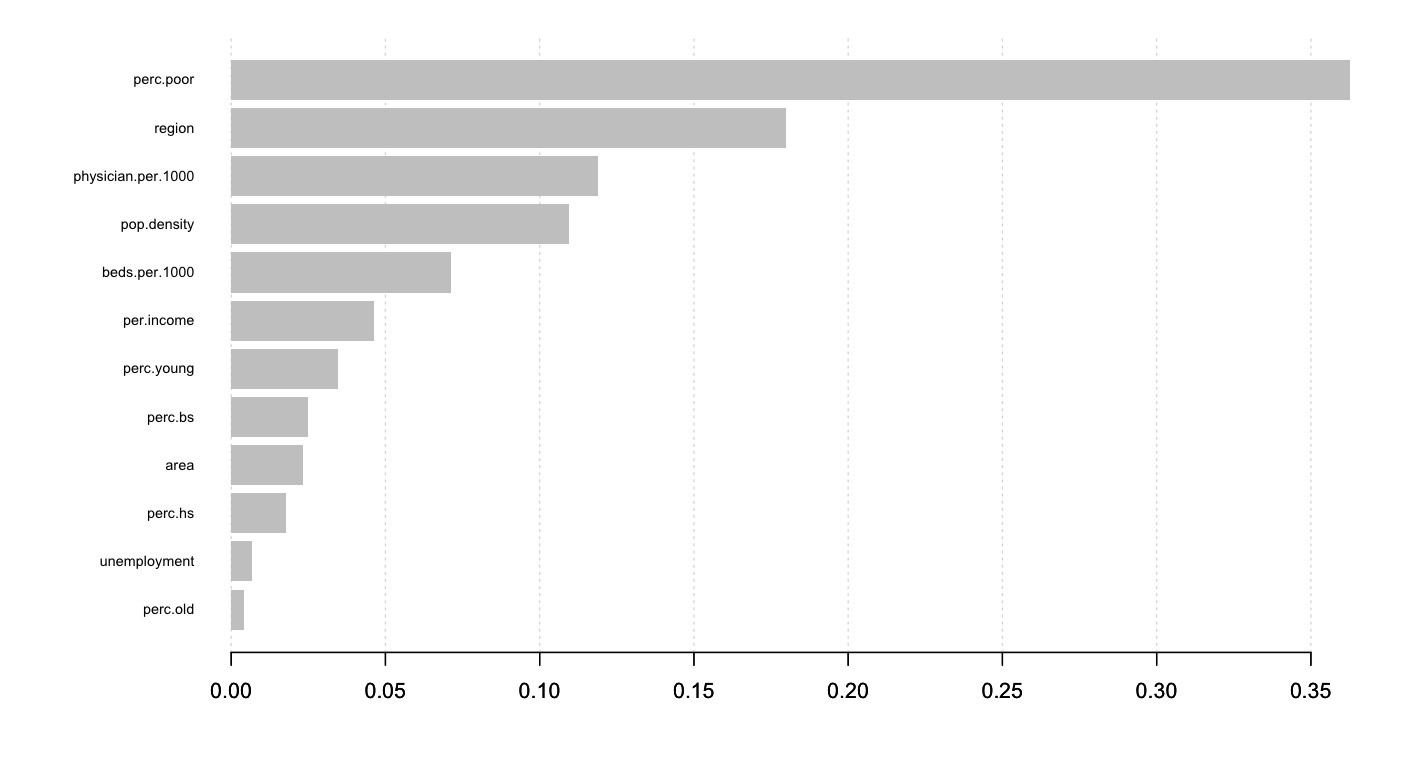
\includegraphics[width=5in]{ada5.jpg}}
\end{center}
\end{frame}


\begin{frame}[fragile]
\frametitle{Kings County with other counties in US}
We can see that among the several variables we focus on, Kings county has a significant high population density, which might be one of the reasons why Kings County has a high crime rate.
\begin{center}
  \makebox[\linewidth]{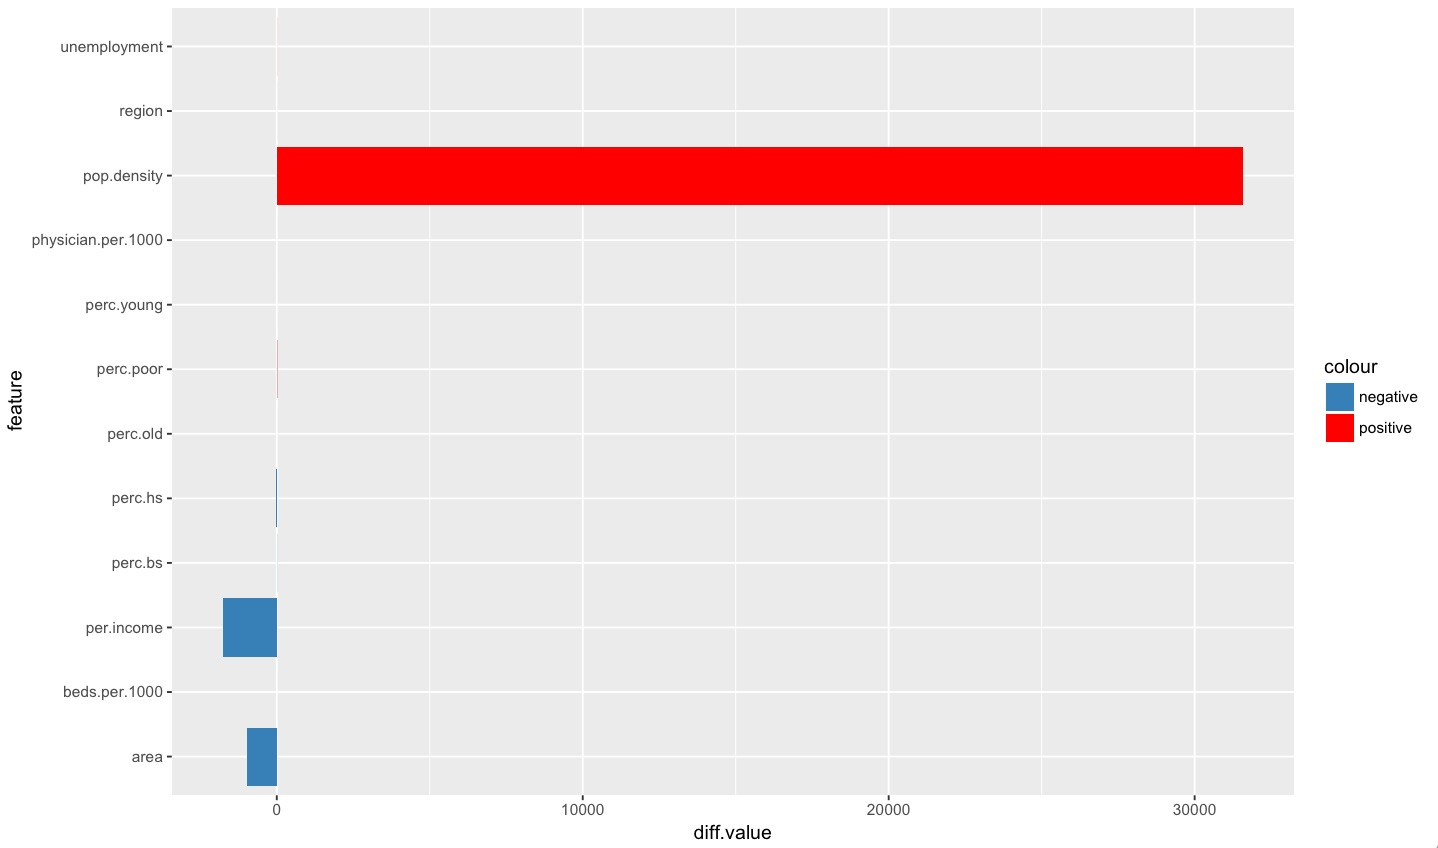
\includegraphics[width=3.5in]{ada6.jpg}}
\end{center}
\end{frame}



\begin{frame}[fragile]
\frametitle{Kings County with other counties in NY}
Assuming counties that are adjacent to each other might have more similarities, we see the difference between Kings County and other counties in the State of NY.
\begin{center}
  \makebox[\linewidth]{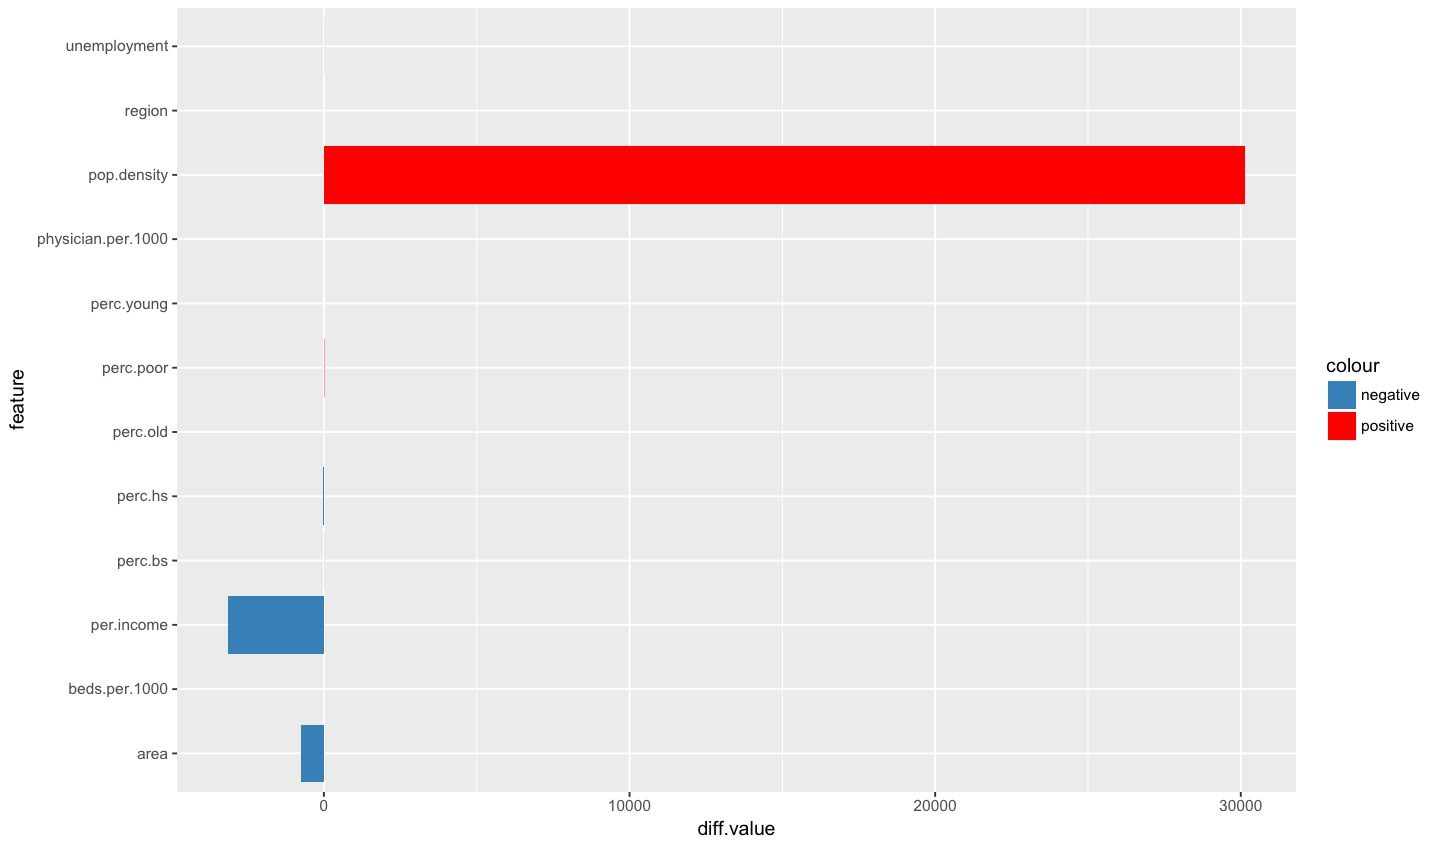
\includegraphics[width=3.5in]{ada7.jpg}}
\end{center}
We can see that the biggest difference is still population density. Thus, we analyze population density's impact on crime rate.
\end{frame}


\begin{frame}[fragile]
\frametitle{Regression on counties including Kings}
\begin{center}
  \makebox[\linewidth]{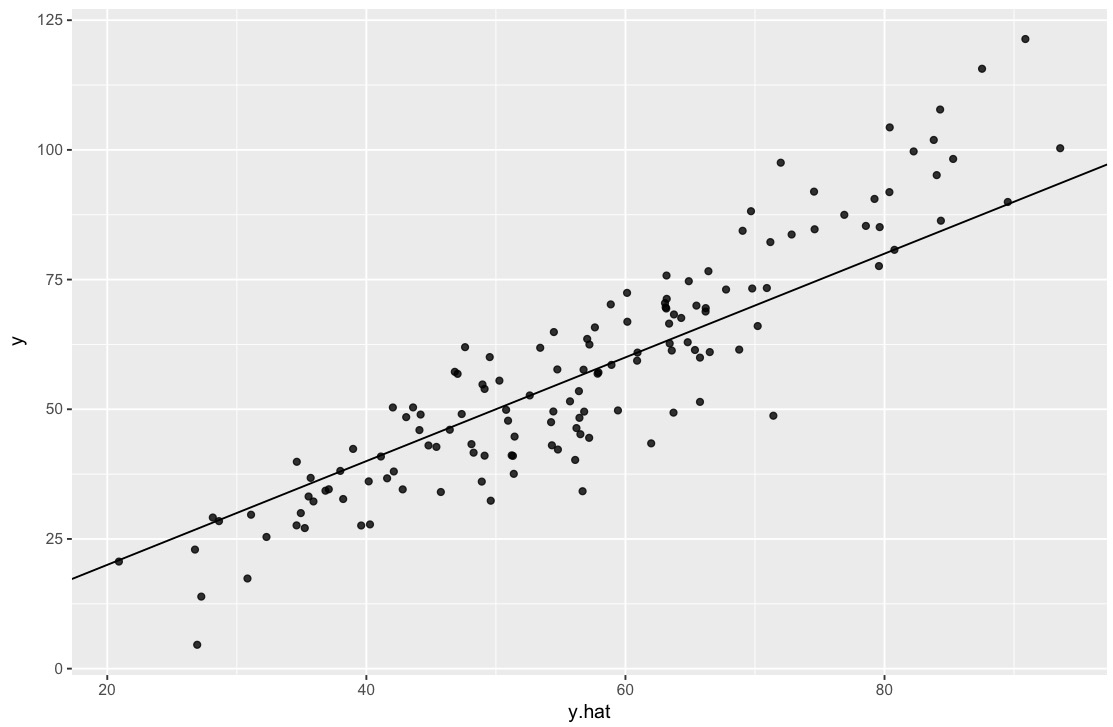
\includegraphics[width=4in]{ada8.jpg}}
\end{center}
\end{frame}

\begin{frame}[fragile]
\frametitle{Important Features}
\begin{center}
  \makebox[\linewidth]{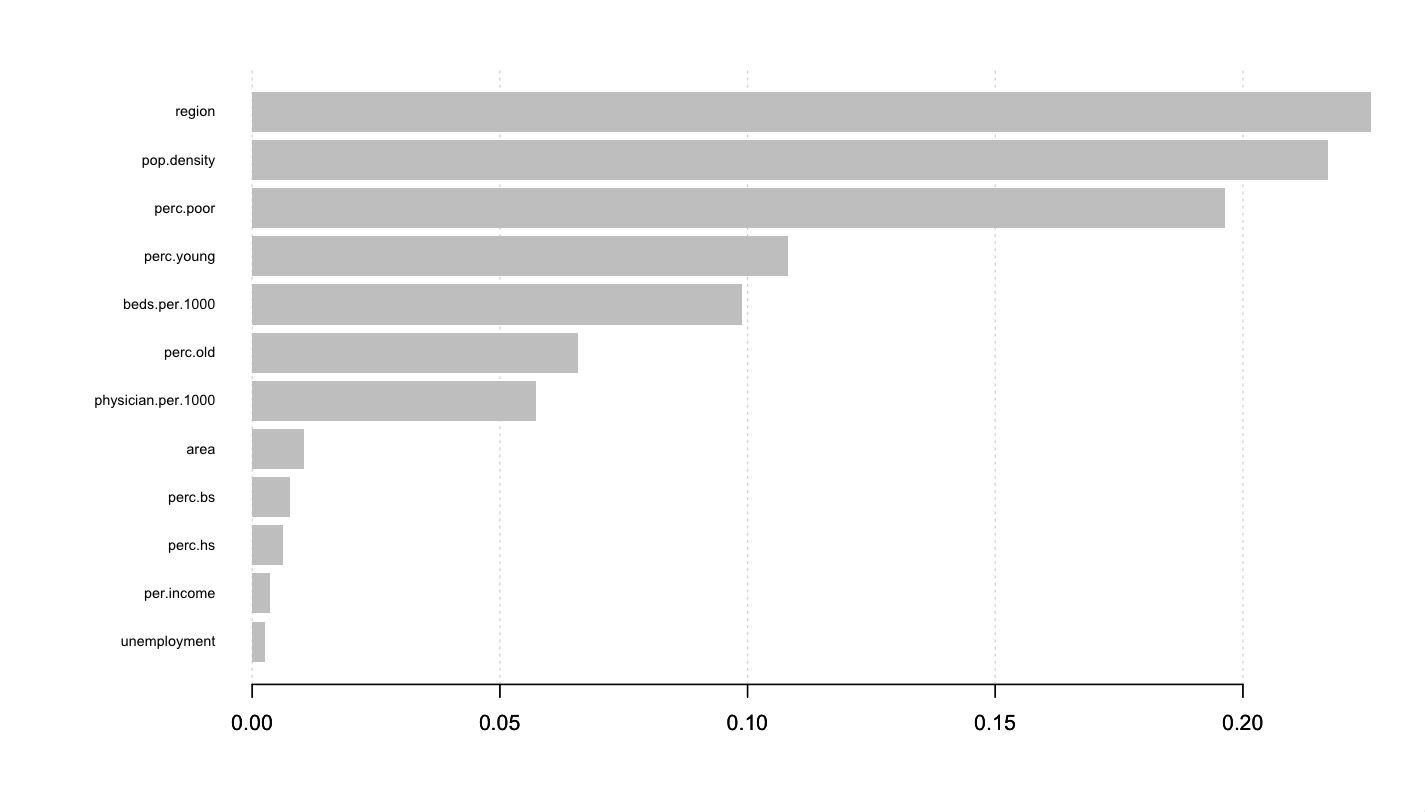
\includegraphics[width=5in]{ada9.jpg}}
\end{center}
\end{frame}


\begin{frame}[fragile]
\frametitle{Population Density}
\begin{center}
  \makebox[\linewidth]{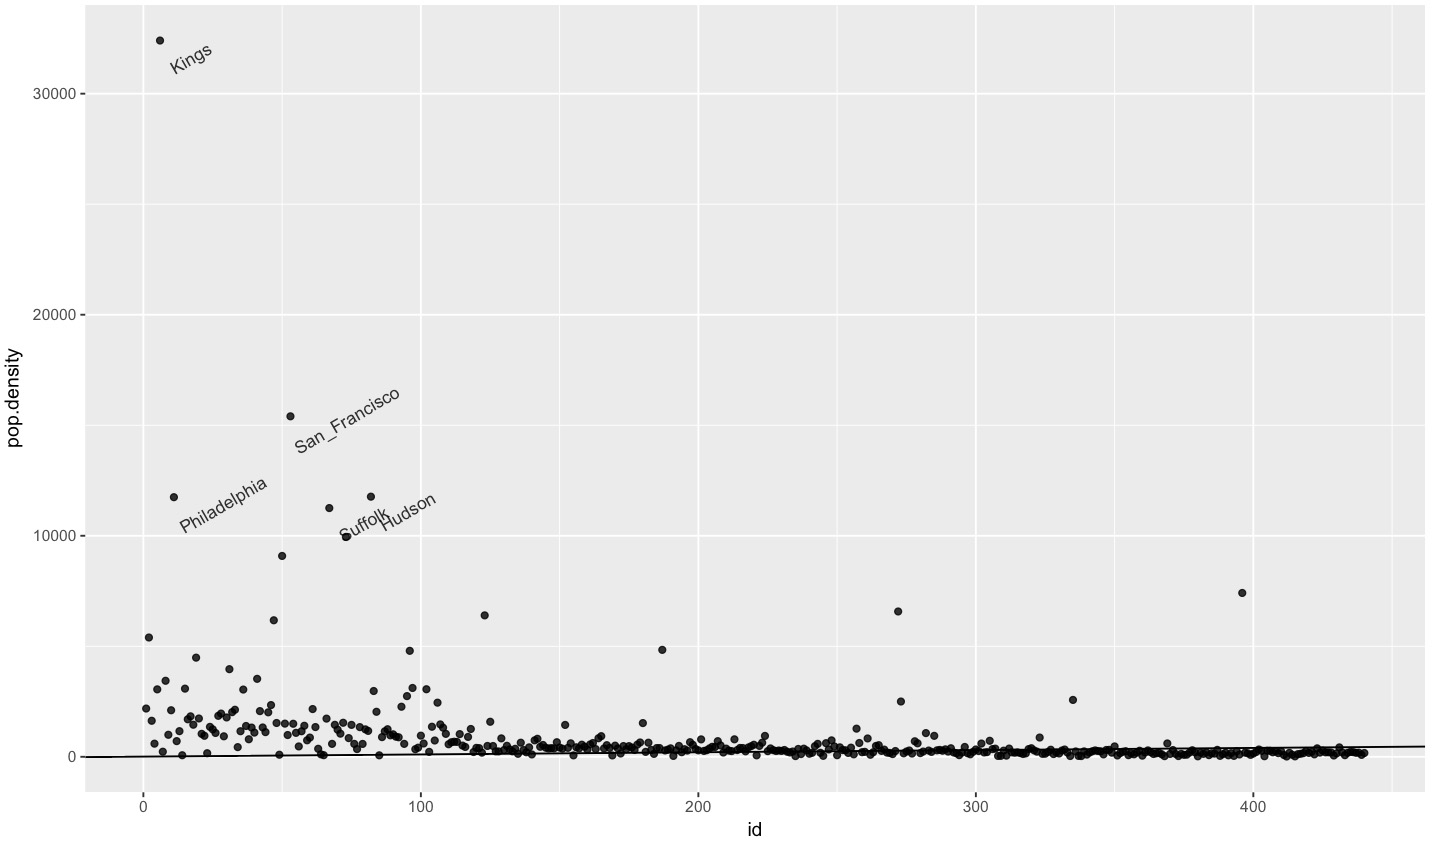
\includegraphics[width=5in]{ada10.jpg}}
\end{center}
\end{frame}

\section{Suggestions and Improvements}
\begin{frame}{Suggestions\dots{}}
Based on the value of the parameters, we give the following suggestions to the officials of Kings County:
\begin{itemize}
\item 1. Control the population of King's County
\item 2. Adopt better policy to raise the level of people's life quality.
\item 3.
\end{itemize}

\end{frame}

\begin{frame}{Improvements\dots{}}
The Regression Model above may be fit for most counties in America, but it doesn't reveal the hidden reasons for the extremely high crime rate in some counties.

\begin{block}{Social Economic Reasons}
"Crime rates spiked in the 1980s and early 1990s as \textbf{the crack epidemic} hit the city."\\
\bigbreak
\small{Crime in New York City - Wikipedia\\ \url{http://bit.ly/2oYXTQQ}}
\end{block}
% The LaTeX wikibook is also a good source of info, e.g.
% http://en.wikibooks.org/wiki/LaTeX/Chemical_Graphics

\begin{block}{Food For Thought}
"New York City Crime in the Nineties - The New Yoker"\\
\bigbreak
\small{\url{http://bit.ly/2os9ZTQ}}
\end{block}

\end{frame}


\end{document}
%\url{www.overleaf.com/help}




ggplot(data = melted_cormat, aes(Var2, Var1, fill = value))+
 geom_tile(color = "white")+
 scale_fill_gradient2(low = "blue", high = "red", mid = "white",
   midpoint = 0, limit = c(-1,1), space = "Lab",
   name="Pearson\nCorrelation") +
  theme_minimal()+
 theme(axis.text.x = element_text(angle = 45, vjust = 1,
    size = 12, hjust = 1), axis.title.x=element_blank(), axis.title.y=element_blank())+
 coord_fixed()
